\section{相关技术与理论基础}\label{chap:theory}

本章介绍与系统设计和实现密切相关的理论基础和技术栈，包括图像隐写术的基本概念、可证安全隐写理论、Pulsar 和 SparSamp 两种隐写算法的工作原理、端到端加密机制以及系统开发涉及的关键技术。

\subsection{图像隐写术概述}

图像隐写术是指将秘密信息嵌入到数字图像中，使得含密图像（Stego Image）在视觉上与原始载体图像（Cover Image）无显著差异，从而实现隐蔽通信的技术\supercite{fridrich2009steganography}。根据嵌入域的不同，图像隐写方法主要分为以下几类：

\subsubsection{空间域隐写}

空间域隐写直接修改图像像素值来嵌入信息。最经典的是 LSB（Least Significant Bit）替换方法，将秘密信息的每一比特替换载体图像对应像素的最低有效位\supercite{chan2004hiding}。该方法实现简单、嵌入容量大，但由于直接改变了像素的统计分布，容易被隐写分析检测。

为降低嵌入失真，研究者提出了多种自适应隐写方法。HUGO\supercite{pevny2010using}通过最小化高阶残差统计量的变化来选择嵌入位置；WOW\supercite{holub2012designing}利用小波变换获取像素权重，优先在纹理复杂区域嵌入；S-UNIWARD\supercite{holub2014universal}在空间域和JPEG域统一使用方向滤波器组计算嵌入代价，是目前抗检测能力较强的方法之一。

\subsubsection{变换域隐写}

变换域隐写在图像经过某种数学变换（如离散余弦变换 DCT、离散小波变换 DWT）后的系数上嵌入信息。典型代表是 JPEG 域隐写，如 F5 算法\supercite{westfeld2001f5}通过减小DCT系数的绝对值嵌入信息，nsF5\supercite{fridrich2007statistically}进一步避免了收缩问题，J-UNIWARD\supercite{holub2014universal}则实现了最优的嵌入代价分配。

\subsubsection{基于生成模型的隐写}

与修改已有图像不同，基于生成模型的隐写方法直接在图像生成过程中嵌入信息，不需要已有的载体图像。这类方法利用深度生成模型（如 GAN、VAE、Flow、扩散模型）采样过程中的随机性嵌入秘密信息，使得含密图像与模型正常输出的图像在分布上完全一致，从根本上消除了隐写痕迹\supercite{de2022perfectly}。

\subsection{可证安全隐写理论}

\subsubsection{信息论安全模型}

可证安全隐写（Provably Secure Steganography）的理论基础源于 Cachin\supercite{cachin2004information}和 Hopper 等人\supercite{hopper2009provably}的工作。其核心思想可以用信息论的语言形式化描述：

设 $P_C$ 表示正常载体（Cover）的分布，$P_S$ 表示含密载体（Stego）的分布。隐写系统的安全性通过两个分布之间的统计距离来度量。常用的度量指标为 KL 散度（Kullback-Leibler Divergence）：

\begin{equation}\label{eq:kl}
    D_{KL}(P_S \| P_C) = \sum_{x} P_S(x) \log \frac{P_S(x)}{P_C(x)}
\end{equation}

\subsubsection{Cachin 安全准则}

Cachin\supercite{cachin2004information}提出了基于 KL 散度的隐写安全性分级：

\begin{itemize}
    \item \textbf{完美安全（$\epsilon$-secure，$\epsilon=0$）}：若 $D_{KL}(P_S \| P_C) = 0$，即含密载体与正常载体的分布完全一致，则任何检测器都无法以优于随机猜测的概率检测隐写行为。
    \item \textbf{近似安全（$\epsilon$-secure，$\epsilon > 0$）}：若 $D_{KL}(P_S \| P_C) \leq \epsilon$，其中 $\epsilon$ 为一个很小的正数，则隐写系统具有近似安全性。
\end{itemize}

实现完美安全的关键在于：隐写编码过程不能对载体分布引入任何偏差。基于生成模型的隐写方案通过在模型的采样过程中嵌入信息，天然地满足了这一要求——因为含密图像也是由同一个生成模型产生的，其分布与正常生成图像完全一致。

\subsection{Pulsar 算法原理}\label{sec:pulsar}

Pulsar\supercite{jois2024pulsar}是一种基于扩散模型的可证安全图像隐写算法，由 Jois、Beck 和 Kaptchuk 于 2024 年提出，发表于 ACM CCS 2024。该算法通过控制逆向去噪过程中最后一步调度器的方差噪声来源实现隐写嵌入。在实际系统中，Pulsar 使用 DDIM（Denoising Diffusion Implicit Models）\supercite{song2020denoising}采样器以 50 步完成图像生成，相比原始 DDPM 的 1000 步大幅降低了计算开销，同时保持了生成质量。

\subsubsection{扩散模型基础}

扩散模型\supercite{ho2020denoising}是一类通过逐步去噪过程生成数据的深度生成模型，近年来在图像生成领域取得了突破性进展\supercite{rombach2022high}，主要包含前向扩散过程和逆向去噪过程：

\textbf{前向扩散过程}：从真实数据 $x_0$ 出发，逐步添加高斯噪声，经过 $T$ 步后得到近似纯噪声 $x_T \sim \mathcal{N}(0, I)$：

\begin{equation}\label{eq:forward}
    q(x_t | x_{t-1}) = \mathcal{N}(x_t; \sqrt{1-\beta_t} x_{t-1}, \beta_t I)
\end{equation}

其中 $\beta_t$ 为预定义的噪声调度参数。

\textbf{逆向去噪过程}：训练一个神经网络 $\epsilon_\theta$ 预测每一步的噪声，从纯噪声 $x_T$ 开始逐步去噪恢复图像：

\begin{equation}\label{eq:reverse}
    p_\theta(x_{t-1} | x_t) = \mathcal{N}(x_{t-1}; \mu_\theta(x_t, t), \sigma_t^2 I)
\end{equation}

其中 $\mu_\theta$ 由模型预测的噪声计算得出，$\sigma_t$ 为方差系数。每步去噪都需要引入随机噪声 $z_t \sim \mathcal{N}(0, I)$。扩散模型的前向加噪与逆向去噪过程如\cref{fig:diffusion_process}所示。

\begin{figure}[htb!]
    \centering
    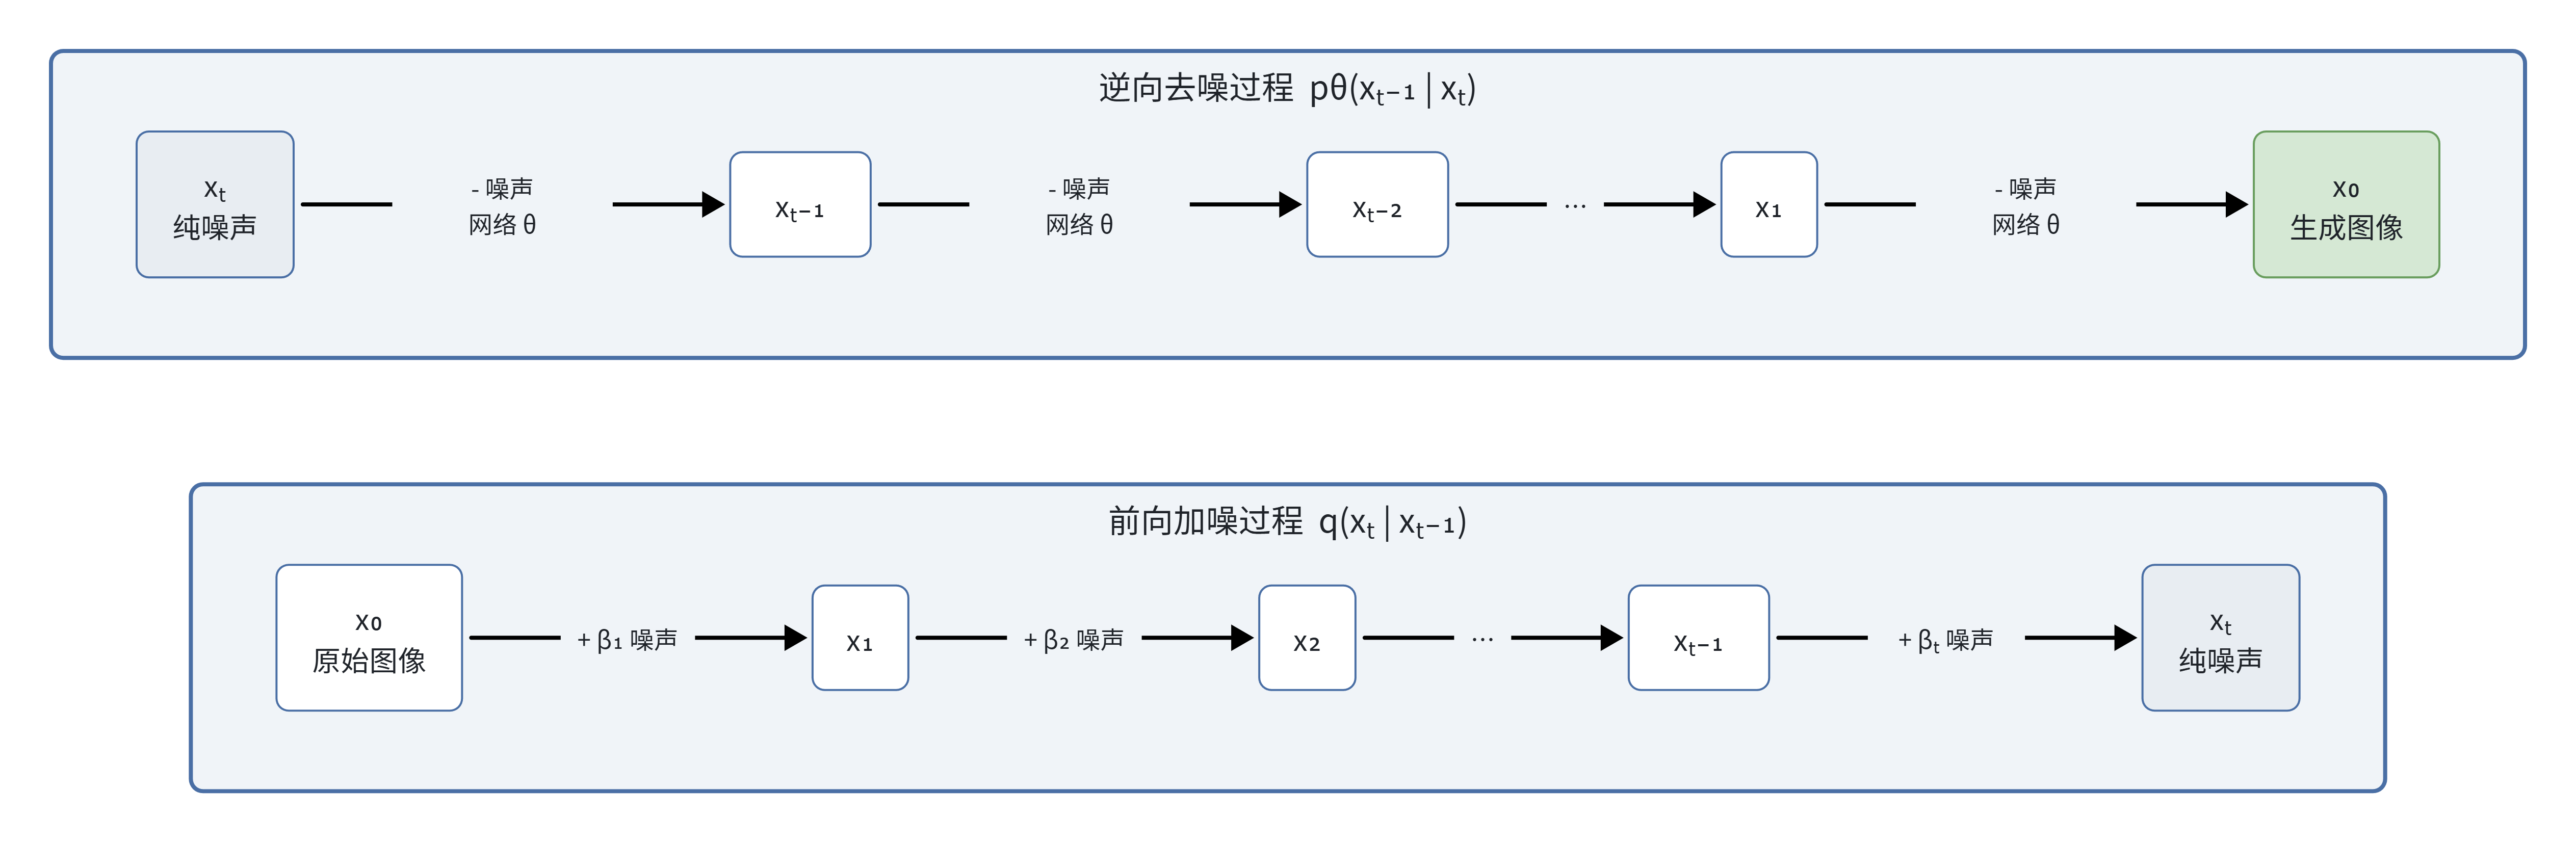
\includegraphics[width=0.9\textwidth]{img/ch2_diffusion_process.png}
    \caption{扩散模型前向加噪与逆向去噪过程}
    \label{fig:diffusion_process}
\end{figure}

\subsubsection{Pulsar 隐写编码原理}

Pulsar 的核心思想是：利用扩散模型逆向去噪过程中最后一步调度器添加的方差噪声（variance noise）作为隐写信道。发送方和接收方共享密钥 $K$，将其解析为三个 PRG 密钥：种子密钥 $k_s$ 和两个参考密钥 $k_0$、$k_1$。$k_s$ 用于同步前 $t-2$ 步去噪过程中的所有随机性，使双方生成完全相同的中间状态；$k_0$ 和 $k_1$ 则分别用于在最后一步调度器中采样不同的高斯噪声序列。

Pulsar 的嵌入过程分为离线阶段和在线阶段：

\begin{enumerate}
    \item \textbf{离线阶段——模型同步}：使用 $k_s$ 确定性地执行前 $t-2$ 步逆向去噪，生成中间状态 $s_{t-2}$。对该状态进行试编码，分别使用 $k_0$ 和 $k_1$ 生成两幅参考图像 img$_0$ 和 img$_1$，将两幅图像之间的像素差异按幅值划分为 $u$ 个桶（bucket），每个桶对应一个差异区域，根据各区域的实际误码率选择合适的纠错码参数。
    \item \textbf{离线阶段——消息预编码}：使用选定的纠错码对秘密消息 $m$ 进行编码，得到扩展后的比特序列 $m_{\text{ECC}}$。
    \item \textbf{在线阶段——噪声采样}：对 $m_{\text{ECC}}$ 中的每一比特 $m_{\text{ECC}}[j]$，若其值为 0，则使用密钥 $k_0$ 采样该像素位置的方差噪声 $r_{t-1}[j]$；若为 1，则使用密钥 $k_1$ 采样。
    \item \textbf{在线阶段——图像生成}：使用编码后的噪声向量 $r_{t-1}$ 执行第 $t-1$ 步调度器，再经确定性的最终步生成含密图像 img。
\end{enumerate}

上述过程的核心在于：每一比特消息通过选择不同的 PRG 密钥来控制对应像素的方差噪声来源。由于 $k_0$ 和 $k_1$ 产生的噪声均服从相同的高斯分布，含密图像的统计特性与正常生成图像不可区分，满足可证安全性。Pulsar 支持离线-在线分离，前 $t-2$ 步的模型推理和区域估计可在消息未知时预先完成，实际编码时仅需执行最后两步调度器和纠错编码。

Pulsar 嵌入流程如\cref{fig:pulsar_embed}所示。

\begin{figure}[htb!]
    \centering
    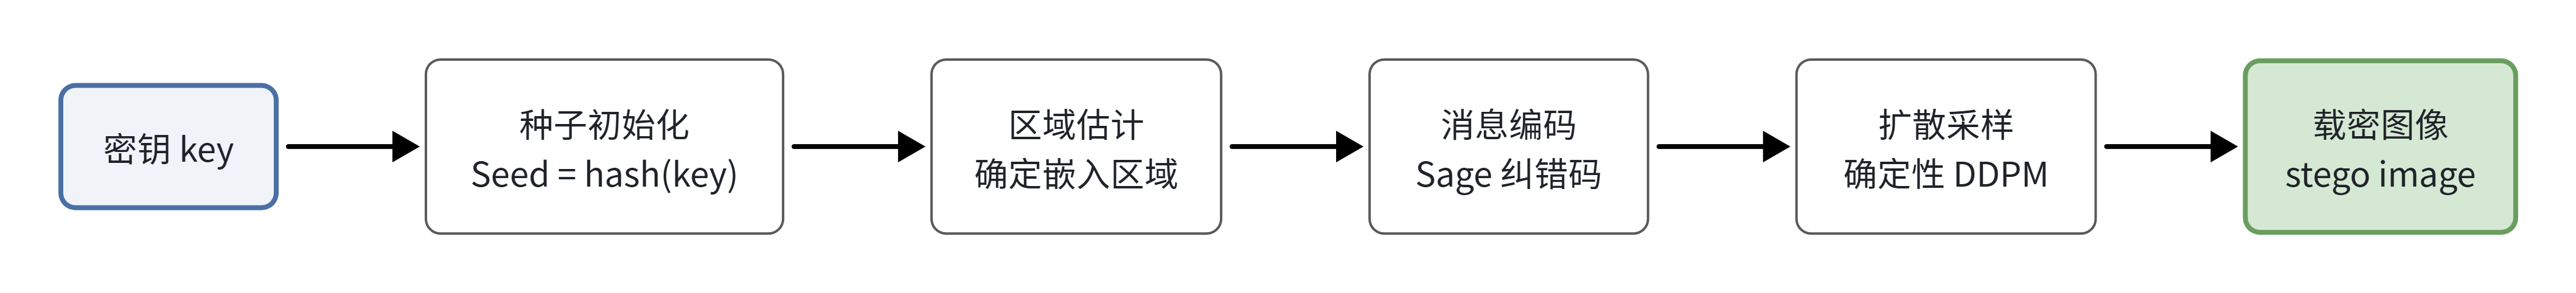
\includegraphics[width=0.85\textwidth]{img/ch2_pulsar_embed.png}
    \caption{Pulsar 隐写嵌入流程}
    \label{fig:pulsar_embed}
\end{figure}

\subsubsection{Pulsar 消息提取}

提取过程与嵌入过程对称：

\begin{enumerate}
    \item \textbf{离线阶段}：接收方使用 $k_s$ 执行前 $t-2$ 步去噪，得到与发送方一致的中间状态 $s_{t-2}$。然后分别使用 $k_0$ 和 $k_1$ 采样最后一步的方差噪声，生成参考图像 img$_0$ 和 img$_1$。
    \item \textbf{在线阶段——比特恢复}：对含密图像 img 的每个编码像素 $j$，计算 $|\text{img}[j] - \text{img}_0[j]|$ 与 $|\text{img}[j] - \text{img}_1[j]|$ 的大小，取距离更近的一方对应的比特值作为恢复值。
    \item \textbf{消息解码}：对恢复的比特序列 $m_{\text{ECC}}$ 执行纠错码的恢复算法，还原原始秘密消息 $m$。
\end{enumerate}

Pulsar 提取流程如\cref{fig:pulsar_extract}所示。

\begin{figure}[htb!]
    \centering
    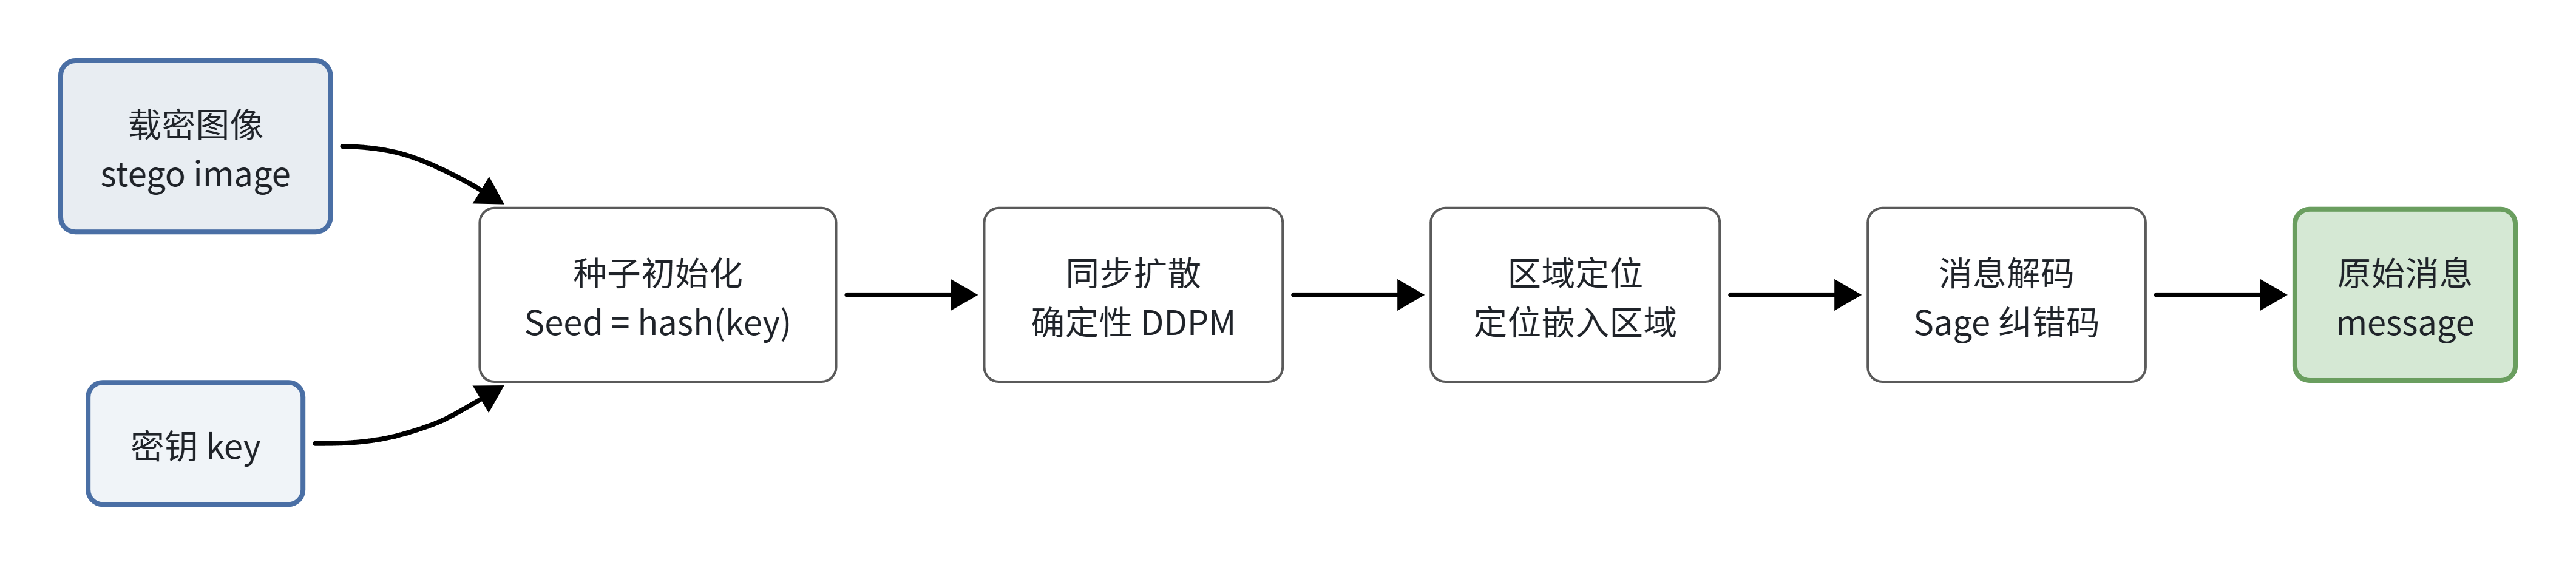
\includegraphics[width=0.85\textwidth]{img/ch2_pulsar_extract.png}
    \caption{Pulsar 消息提取流程}
    \label{fig:pulsar_extract}
\end{figure}

\subsubsection{纠错编码机制}

Pulsar 的信道可建模为二进制对称信道（BSC$_p$），其误码率因图像区域而异。原论文采用二进制级联码（concatenated code）实现变码率纠错：外码为 Reed-Solomon 码，内码为通过手工搜索和经验测试确定的短二进制码，使其在给定 BSC$_p$ 上的解码错误概率尽可能低且码率接近信道容量 $1 - H_2(p)$。

系统根据差异区域的误码率逐区域选择纠错码：从低误码率区域开始，为每个区域分配码率匹配的级联码；当某一区域的误码率过高、超出可用纠错码的纠错能力时，停止在该区域编码。这一策略充分利用了图像中高细节区域的低误码特性，避免了低细节背景区域的高误码拖累整体容量。实验表明，该方法在 256$\times$256 像素图像上平均可嵌入 320--613 字节明文信息。

\subsection{SparSamp 算法原理}\label{sec:sparsamp}

SparSamp\supercite{wang2025sparsamp}是一种基于稀疏采样（Sparse Sampling）的可证安全隐写算法，其核心思想是通过消息驱动采样（Message-Driven Sampling）将秘密消息嵌入生成模型的采样过程中。与基于算术编码的方法不同，SparSamp 通过将消息段与伪随机数进行模加法结合，生成消息导出随机数（Message-derived Random Number, MRN），并利用 MRN 从概率分布中采样 token。当多个 MRN 采样到同一 token 导致解码歧义时，SparSamp 通过逐步缩小候选消息集合来增大相邻 MRN 之间的采样间隔，实现稀疏采样，从而消除歧义。该方法严格保持原始概率分布不变，且在每步采样中仅引入 $O(1)$ 的额外计算复杂度。本系统基于 IDDPM（Improved Denoising Diffusion Probabilistic Models）\supercite{nichol2021improved}的 P2-weighting 框架实现了 SparSamp 的图像隐写版本。

\subsubsection{P2-weighting 框架}

P2-weighting 是 IDDPM 的一种训练策略，通过为不同噪声水平分配不同的训练权重来提升生成质量。SparSamp 使用的 UNet 模型具有以下特征：

\begin{itemize}
    \item \textbf{输出通道}：6 通道，其中 3 通道预测噪声 $\epsilon$，3 通道预测 $v$ 插值参数。
    \item \textbf{模型架构}：基础通道数 128，通道倍增因子 $(1,1,2,2,4,4)$，注意力分辨率 $(16,)$。
    \item \textbf{图像尺寸}：$256 \times 256$ 像素。
    \item \textbf{方差学习}：通过 $v$ 参数化实现 $\sigma$ 的学习。
\end{itemize}

\subsubsection{SparSamp 嵌入流程}

SparSamp 的嵌入过程基于消息驱动采样机制，主要分为以下步骤：

\begin{enumerate}
    \item \textbf{密钥派生}：对共享密钥 $K$ 计算 SHA-256 哈希，前 4 字节作为扩散采样种子，后 4 字节作为 SparSamp 编码种子。
    \item \textbf{确定性扩散采样}：使用派生的种子设置所有随机数生成器（PyTorch、CUDA、NumPy），确保环境完全确定性。从纯噪声 $x_T$ 出发，经 $N$ 步（默认 10 步）逆向去噪到达 $x_1$。
    \item \textbf{最后一步分布计算}：在 $t=0$ 时刻对 $x_1$ 执行模型前向计算，得到每个像素的高斯分布参数 $(\mu_i, \sigma_i)$，并将连续高斯分布量化为 256 个离散 bin。
    \item \textbf{消息驱动采样}：将消息打包为比特序列（32 位长度头 + UTF-8 载荷），按 $l_m$ 比特一组划分为消息段。对每个像素，将当前消息段通过 $\textsf{bin2num}$ 函数转换为 $[0,1)$ 区间内的数值，与伪随机数 $r_i$ 进行模加法得到 MRN：$r_i(m) = [r_i + \textsf{bin2num}(m)] \bmod 1$。使用 MRN 从该像素的量化分布中采样一个 bin 索引。
    \item \textbf{稀疏采样消歧}：当多个候选消息段的 MRN 采样到同一个 bin 时，记录所有产生相同采样结果的候选 MRN，并在下一个像素的采样中使用这些候选 MRN 继续嵌入。随着候选集合 $N_m$ 的缩小，相邻 MRN 之间的距离 $\frac{1}{N_m}$ 增大，采样变得更加稀疏，从而消除解码歧义，直到候选集合缩小为 1（即消息段被唯一确定）。
    \item \textbf{图像生成}：采样完成后的 bin 索引数组（shape $3 \times 256 \times 256$）转换为像素值，保存为 PNG 图像。
\end{enumerate}

SparSamp 嵌入流程如\cref{fig:sparsamp_embed}所示。

\begin{figure}[htb!]
    \centering
    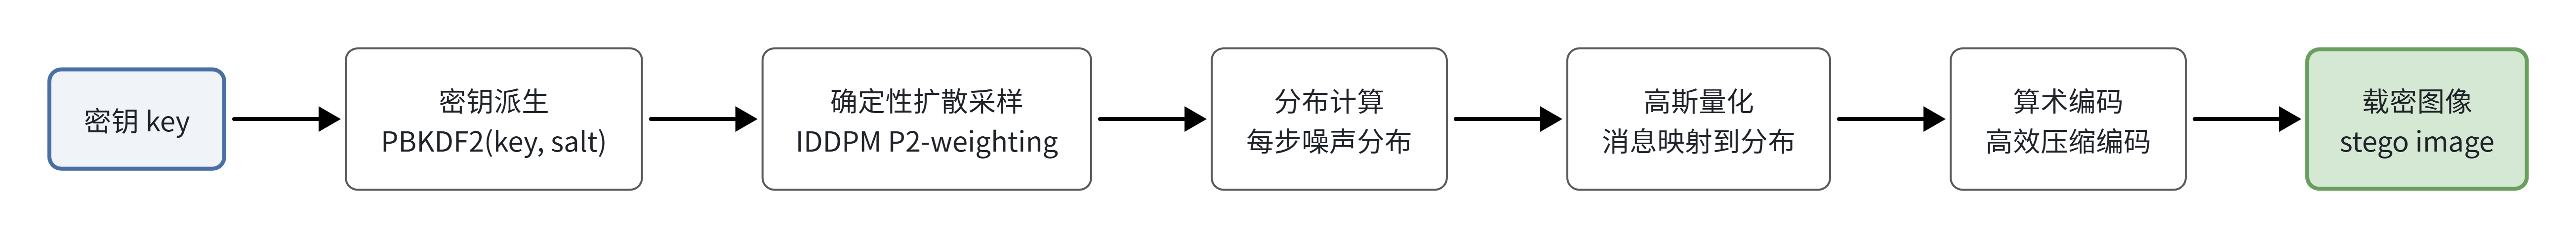
\includegraphics[width=0.85\textwidth]{img/ch2_sparsample_embed.png}
    \caption{SparSamp 嵌入流程}
    \label{fig:sparsamp_embed}
\end{figure}

\subsubsection{SparSamp 提取流程}

提取过程是嵌入的对称操作：使用相同的密钥派生相同的种子，执行相同的扩散采样和分布计算，然后从像素值反向推导出 bin 索引。利用相同的伪随机数序列和 MRN 更新逻辑（$\textsf{sparse}$ 函数），逐步缩小候选消息集合，直到 $N_m=1$ 时即可唯一确定当前消息段的值。提取时先读取 32 位长度头确定消息总长度，再依次恢复各消息段并拼接为完整消息。

\subsubsection{状态缓存机制}

SparSamp 的扩散采样和分布计算耗时较长（约 50 秒），因此系统对每个（模型、密钥）对的计算结果进行缓存。首次请求时执行完整的扩散流程并缓存中间状态（$x_1$、$\mu$、$\sigma$），后续相同（模型、密钥）对的请求直接使用缓存，实现瞬时返回。

\subsection{端到端加密机制}\label{sec:e2ee}

本系统实现了基于对称助记词的端到端加密方案，主要包括密钥派生、消息加密封装和隐写密钥协商三个环节。E2EE 密钥派生层次如\cref{fig:e2ee_keys}所示。

\begin{figure}[htb!]
    \centering
    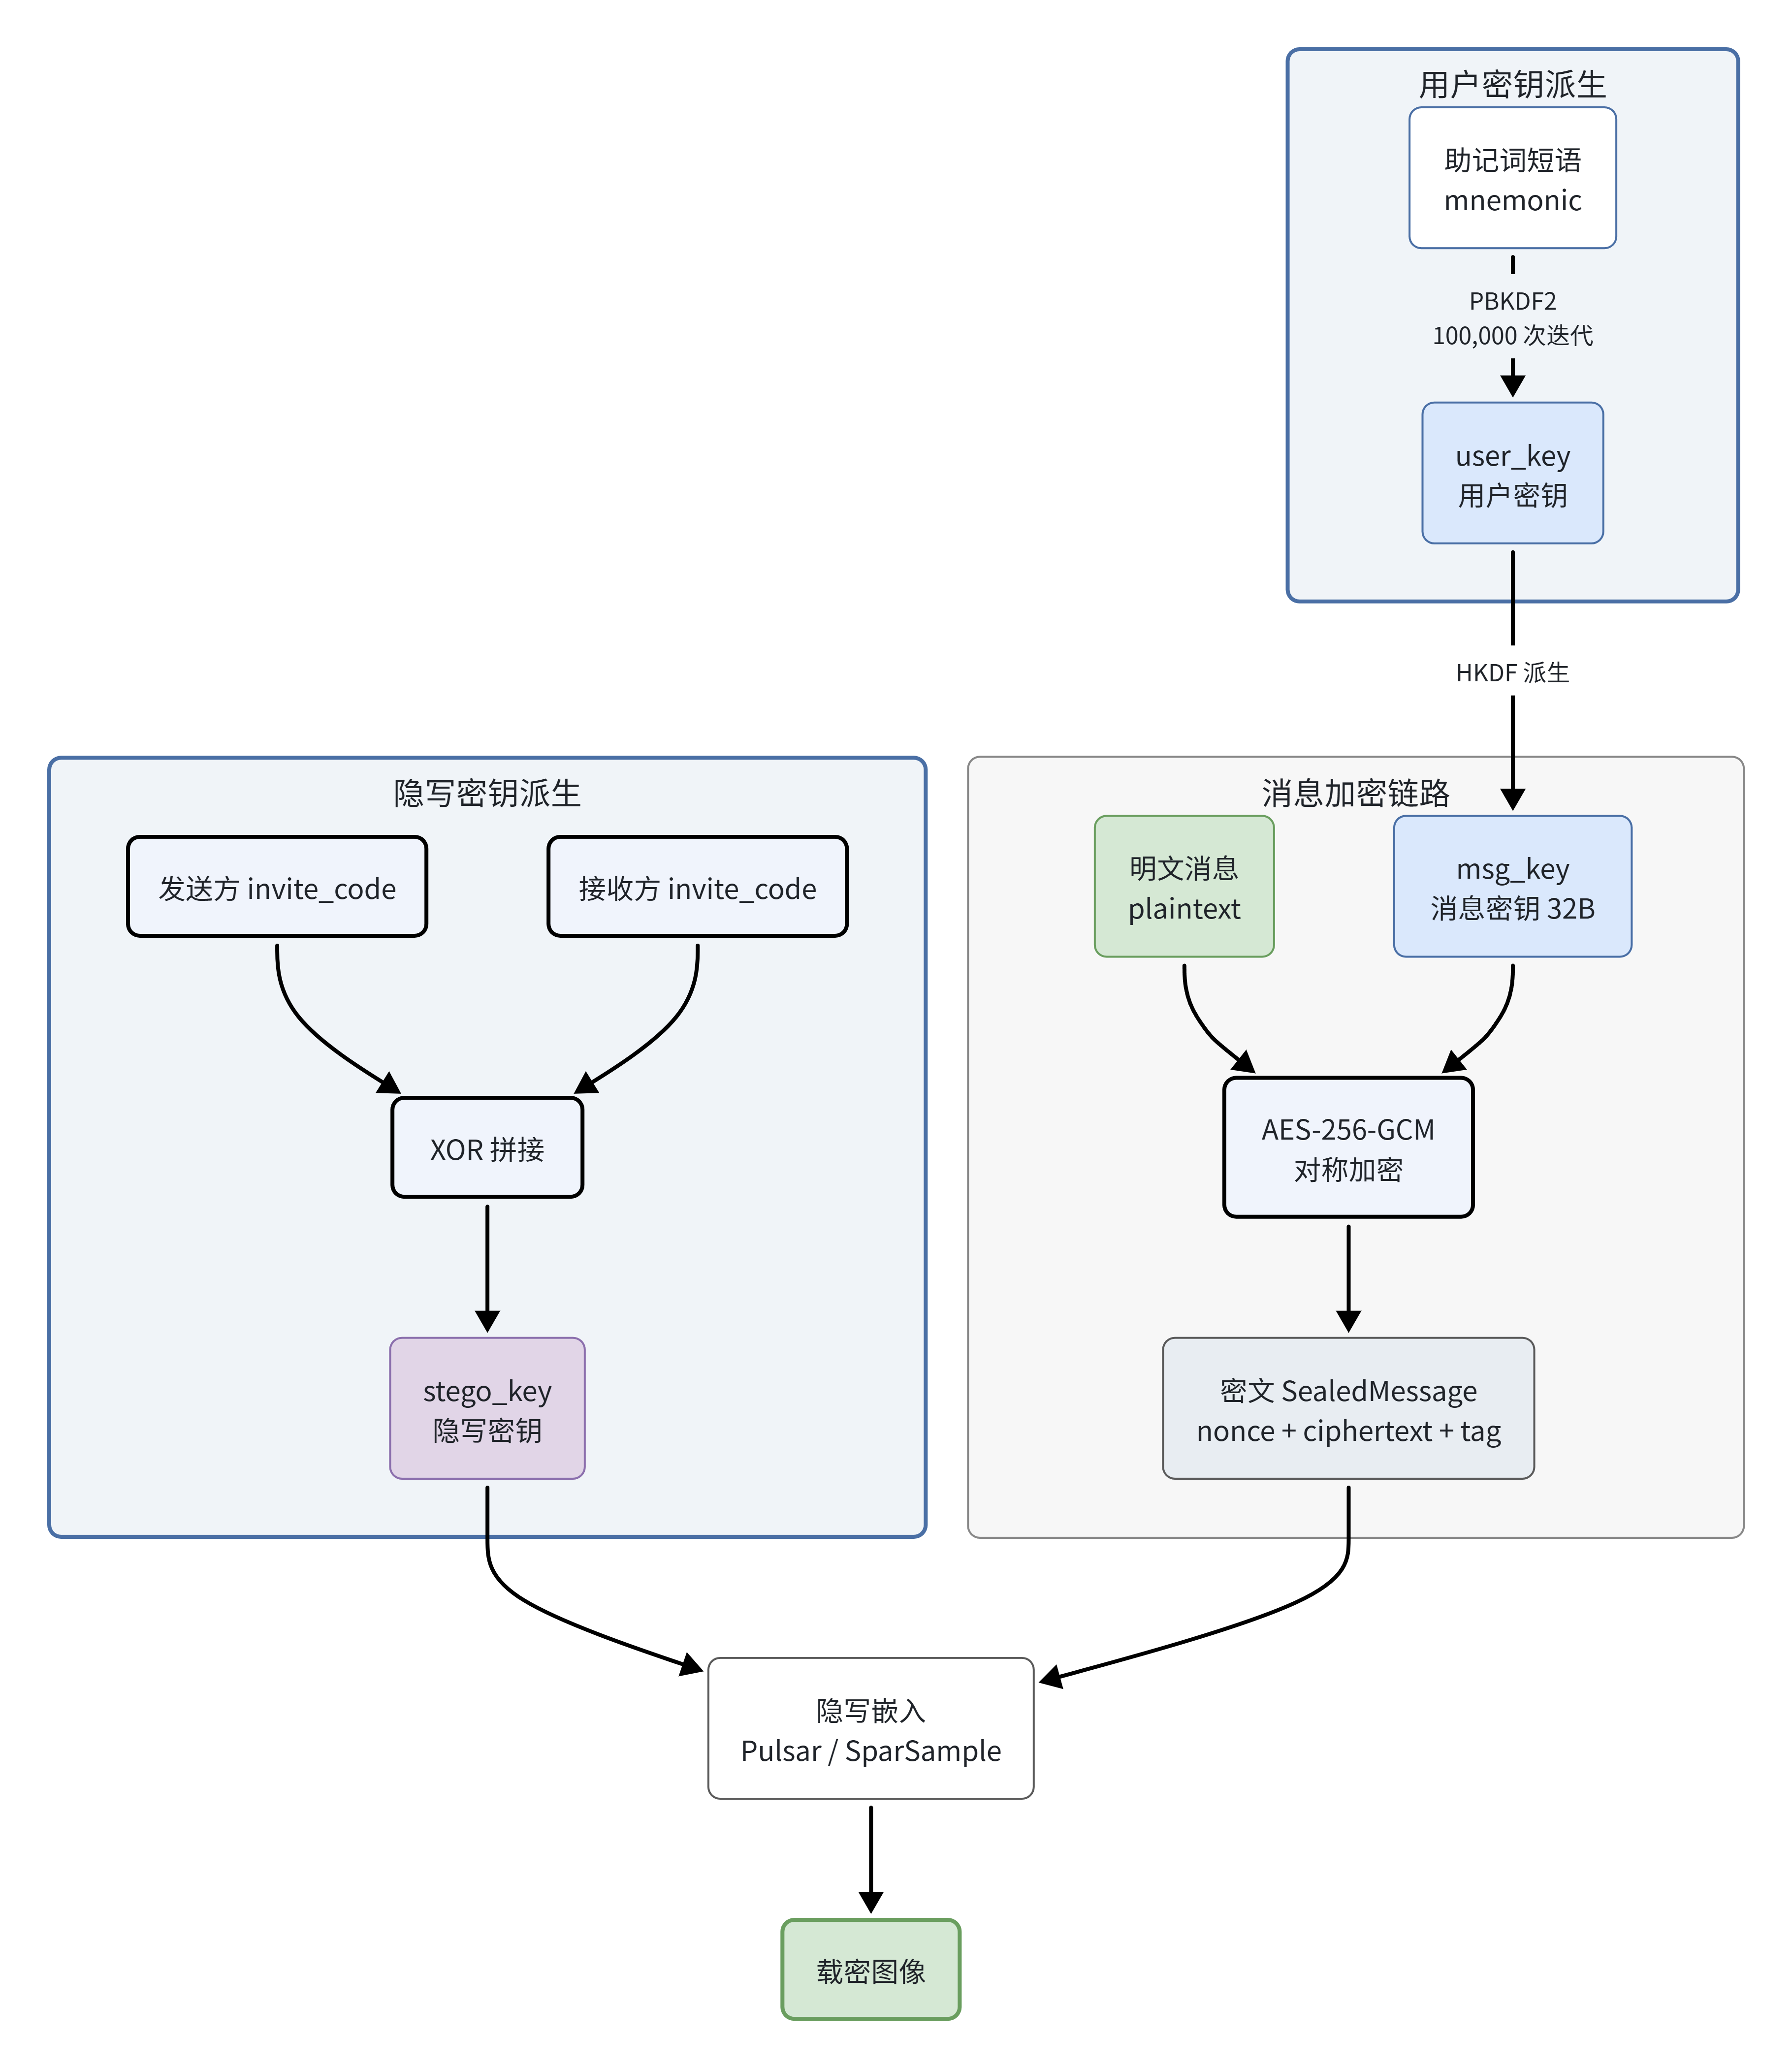
\includegraphics[width=0.85\textwidth]{img/ch2_e2ee_keys.png}
    \caption{E2EE 密钥派生层次}
    \label{fig:e2ee_keys}
\end{figure}

\subsubsection{用户密钥派生}

每个用户持有一个助记词短语（任意字符串），通过 PBKDF2-SHA256 算法派生 256 位用户密钥：

\begin{equation}\label{eq:userkey}
    \text{userKey} = \text{PBKDF2}(\text{phrase}, \text{salt}_s, 100000, 256)
\end{equation}

其中 $\text{salt}_s = \text{"stegochat-seed-v1"}$ 为固定的种子盐值，迭代次数为 100,000 次。派生完成后，计算用户密钥的 SHA-256 指纹（取前 8 字节）用于配对验证：

\begin{equation}\label{eq:fingerprint}
    \text{fingerprint} = \text{SHA-256}(\text{userKey})[0:8]
\end{equation}

指纹以冒号分隔的十六进制格式显示（如 \texttt{a1:b2:c3:d4:e5:f6:a7:b8}），用户可通过对比指纹验证密钥配对的正确性。

\subsubsection{消息密钥协商}

通信双方的用户密钥通过对称的 HKDF-SHA256 算法\supercite{rfc5869}协商出消息密钥。为保证对称性（即 $\text{deriveMkey}(A, B) = \text{deriveMkey}(B, A)$），双方的用户密钥按字典序排列后拼接：

\begin{equation}\label{eq:mkey}
    \text{mkey} = \text{HKDF}(\text{concat}(\min(K_A, K_B), \max(K_A, K_B)), \text{salt}_m, \text{info}, 256)
\end{equation}

其中 $\text{salt}_m = \text{"stegochat-mkey-v1"}$，$\text{info} = \text{"e2ee"}$。消息密钥仅在内存中存在，不进行持久化存储，每次切换聊天对象时重新计算。

\subsubsection{消息加密封装}

消息使用 AES-256-GCM 算法\supercite{nist80038d}加密，封装为 SealedMessage 格式：

\begin{enumerate}
    \item 生成 12 字节随机 nonce。
    \item 使用消息密钥和 nonce 对明文执行 AES-256-GCM 加密，得到密文和 128 位认证标签。
    \item 构造 JSON 信封：$\{v:1, n:\text{base64url}(\text{nonce}), c:\text{base64url}(\text{ciphertext}+\text{tag})\}$。
    \item 将整个 JSON 字符串进行 base64url 编码，得到最终的密封消息字符串。
\end{enumerate}

解封时执行逆操作：base64url 解码、JSON 解析、验证版本号、AES-256-GCM 解密。解密失败时返回空值，支持对未加密的旧格式消息的兼容处理。

\subsubsection{隐写密钥协商}

在隐写聊天模式下，隐写算法需要一个共享密钥作为伪随机数生成器的种子。系统使用通信双方的邀请码进行 XOR 运算来生成隐写密钥：

\begin{equation}\label{eq:stegokey}
    K_{\text{stego}} = \text{inviteCode}_A \oplus \text{inviteCode}_B
\end{equation}

XOR 运算具有对称性（$A \oplus B = B \oplus A$），因此双方无需协商即可独立计算出相同的隐写密钥。邀请码的长度差异通过循环 XOR 处理。生成的密钥以十六进制字符串形式传递给隐写算法的 API 接口。

\subsubsection{隐写聊天的双重保护}

隐写聊天模式下，消息经历"先加密、再隐写"的双重保护流程：

\begin{enumerate}
    \item 发送方使用消息密钥（mkey）对明文执行 AES-256-GCM 加密，得到 SealedMessage。
    \item 将 SealedMessage 字符串作为载荷，使用隐写密钥（$K_{\text{stego}}$）调用隐写嵌入 API。
    \item 隐写算法将加密后的载荷编码到扩散模型生成的图像中，返回含密图像的 base64 数据。
    \item 含密图像通过 WebSocket 发送给接收方。
    \item 接收方使用相同的隐写密钥调用隐写提取 API，得到 SealedMessage 字符串。
    \item 接收方使用消息密钥解封 SealedMessage，还原明文消息。
\end{enumerate}

加密-隐写双重保护的完整流程如\cref{fig:double_protection}所示。

\begin{figure}[htb!]
    \centering
    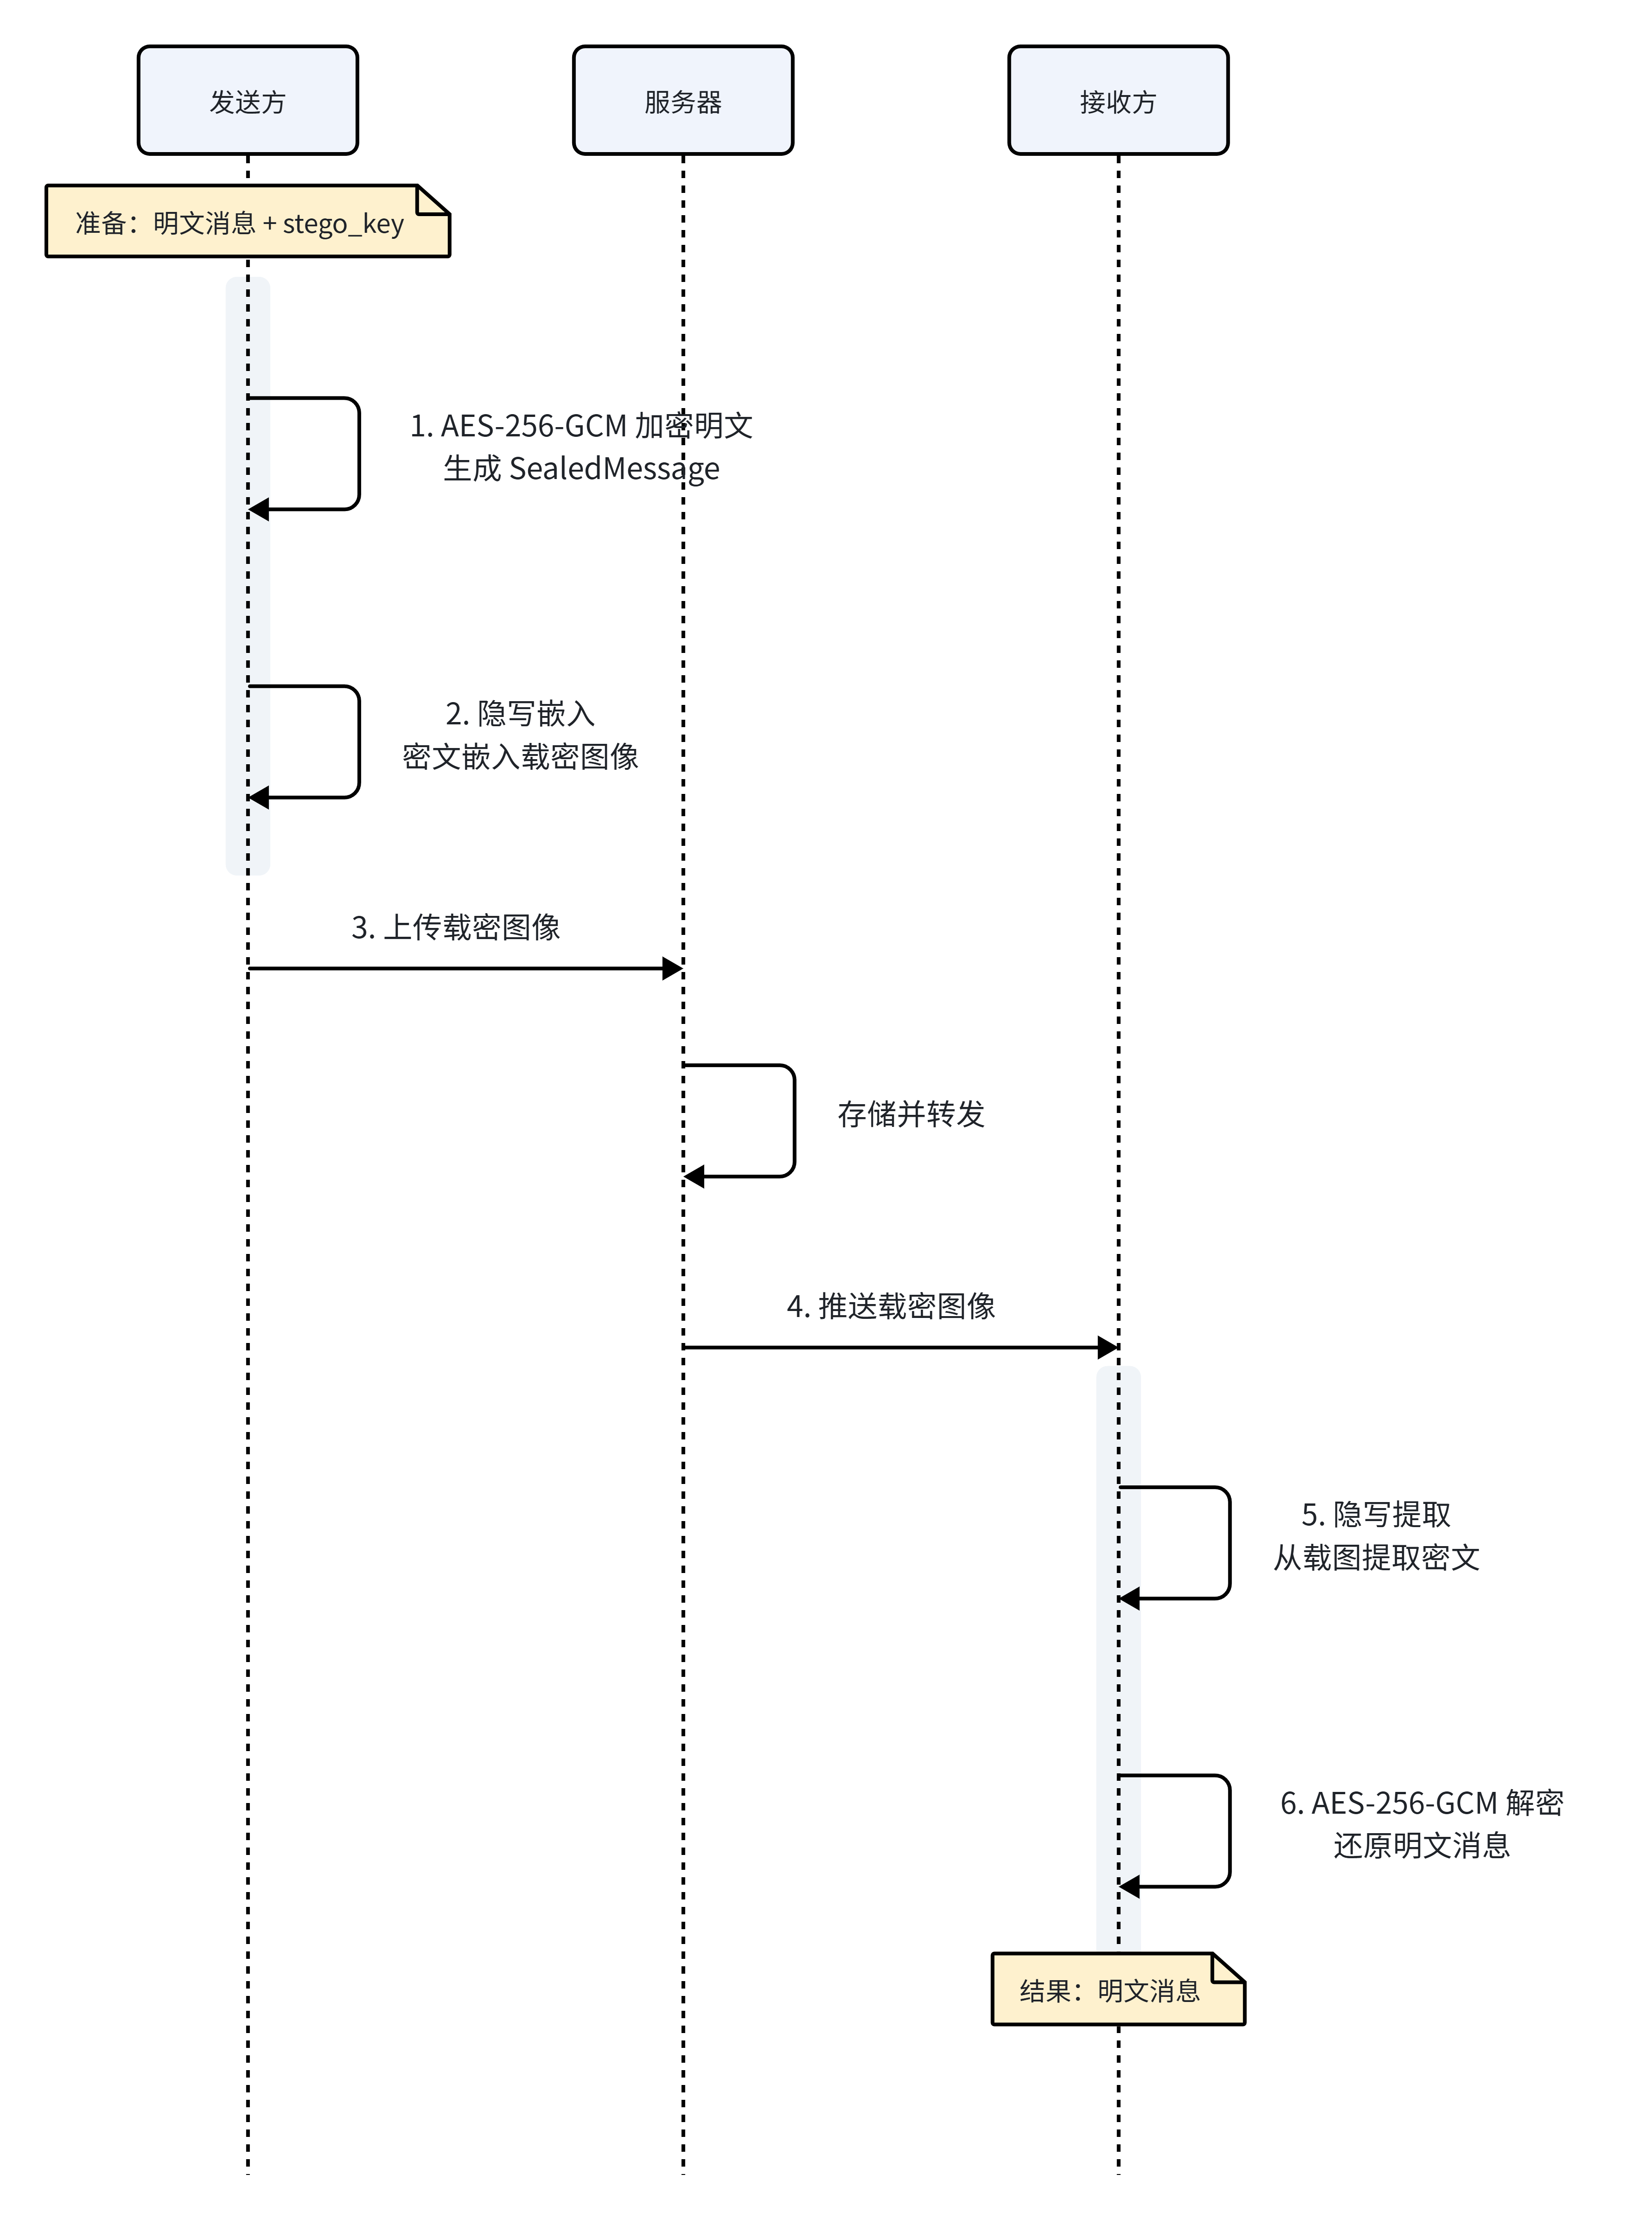
\includegraphics[width=0.85\textwidth]{img/ch2_double_protection.png}
    \caption{加密-隐写双重保护流程}
    \label{fig:double_protection}
\end{figure}

由于隐写嵌入的载荷已经是加密后的密文，即使服务端或攻击者提取出了隐写内容，也无法解密得到原始消息。

\subsection{关键技术栈}\label{sec:techstack}

\subsubsection{FastAPI 框架}

FastAPI\supercite{fastapi}是一个基于 Python 的现代 Web 框架，具有以下特点：

\begin{itemize}
    \item 基于 ASGI（Asynchronous Server Gateway Interface）标准，原生支持异步编程。
    \item 自动生成 OpenAPI 文档和交互式 API 测试界面。
    \item 基于 Python 类型注解的请求参数验证和序列化。
    \item 高性能，与 Node.js 和 Go 等框架性能相当。
\end{itemize}

本系统使用 FastAPI 构建服务端 RESTful API 和 WebSocket 服务，使用 uvicorn 作为 ASGI 服务器。

\subsubsection{WebSocket 协议}

WebSocket 是一种在单个 TCP 连接上进行全双工通信的协议\supercite{fette2011websocket}。与传统的 HTTP 请求-响应模式不同，WebSocket 允许服务端主动向客户端推送消息，适用于实时通信场景。本系统使用 WebSocket 实现即时消息推送、消息状态回执（已发送/已送达/已读）、消息撤回通知、在线状态感知和好友请求通知等功能。

\subsubsection{Jetpack Compose}

Jetpack Compose\supercite{jetpackcompose}是 Google 推出的 Android 现代声明式 UI 框架。与传统的 XML 布局相比，Compose 直接使用 Kotlin 代码描述 UI，支持响应式编程模型，代码更简洁，开发效率更高。本系统的 Android 客户端完全基于 Jetpack Compose 构建，采用 Material 3 Expressive 设计语言。

\subsubsection{Vue.js 3}

Vue.js 3\supercite{vuejs}是一个渐进式 JavaScript 前端框架，采用组合式 API（Composition API）提供更灵活的逻辑复用能力。本系统使用 Vue.js 3 配合 TypeScript 开发 Web 客户端，使用 Pinia 进行状态管理，使用 Vue Router 管理页面路由，使用 Tailwind CSS 实现样式系统。

\subsubsection{本地存储技术}

为实现离线数据持久化，系统在不同平台采用了相应的本地存储方案：

\begin{itemize}
    \item \textbf{SQLite}：服务端使用 SQLite 作为轻量级关系型数据库，通过 aiosqlite 库实现异步操作，启用 WAL 模式提升并发读写性能。
    \item \textbf{Room}：Android 客户端使用 Room 持久化库，它是 SQLite 的抽象层，提供编译时 SQL 验证和与 Kotlin 协程的无缝集成。
    \item \textbf{IndexedDB}：Web 客户端使用浏览器原生 IndexedDB 数据库存储聊天记录和用户数据，通过 idb 库简化操作。
    \item \textbf{DataStore}：Android 客户端使用 Jetpack DataStore 存储 JWT 令牌和用户信息，替代传统的 SharedPreferences。
\end{itemize}

\subsubsection{密码学库}

系统在不同平台使用相应的密码学实现：

\begin{itemize}
    \item \textbf{服务端}：使用 Python 标准库 \texttt{hashlib} 实现 PBKDF2-HMAC-SHA256 密码哈希，使用 \texttt{python-jose} 实现 JWT 令牌的签发和验证。
    \item \textbf{Android 客户端}：使用 Java 标准库 \texttt{javax.crypto} 实现 AES-256-GCM 加密和 HKDF 密钥派生，使用 \texttt{java.security} 实现 PBKDF2。
    \item \textbf{Web 客户端}：使用 Web Crypto API（\texttt{crypto.subtle}）实现所有密码学操作，包括 PBKDF2、HKDF 和 AES-GCM。
\end{itemize}

\subsection{本章小结}

本章介绍了图像隐写术的基本概念和分类，阐述了可证安全隐写的理论基础和 Cachin 安全准则，详细分析了 Pulsar 和 SparSamp 两种隐写算法的嵌入、提取和编码机制，介绍了端到端加密的密钥派生、消息加密封装和隐写密钥协商方案，并介绍了系统开发涉及的关键技术栈。这些理论和技术为后续的系统设计与实现奠定了基础。
